% !TeX root = ./growth_modelling.tex
\documentclass[letterpaper, 11pt]{article}
\usepackage{microtype}
\usepackage[bottom=1in, margin=0.75in]{geometry}
\usepackage{mathpazo}
\usepackage{setspace}
\usepackage{graphicx}
\usepackage[colorlinks=true, allcolors=blue]{hyperref}
\usepackage{amsmath}
\onehalfspacing
\setlength\itemsep{5pt}
\setlength{\footskip}{-10pt}
\title{Constructing a Dynamical Model of Nutrient-Dependent Growth}
\author{Griffin Chure}
\date{\today}
\begin{document}
\maketitle

\section{Theoretical Underpinnings}
\subsection{Translation-Limited Growth}\label{sec:translation_limited_growth}
We begin by considering balanced exponential growth on a single carbon source.
For the time being, we will consider a growth regime where translation is
limiting and we will assume that nutrients are in abundance.  
In this phase of growth, we can consider the formation of protein mass
as the most resource-intensive process and can relate the total 
protein mass of the cell $M$ to the characteristic growth rate $\lambda$ via 
\begin{equation}\label{eq:grow_def}
\frac{dM}{dt} = \lambda M.
\end{equation}
This protein mass $M$ is the product of the pool of ribosomes which catalyze the
formation of peptide bonds via translation. Equation \eqref{eq:grow_def} can be 
cast in terms of the total number of actively translating ribosomes $N_R^{(act.)}$
as 
\begin{equation}
\frac{dM}{dt} = N_R^{(act.)}k_R,
\end{equation}
where $k_R$ represents the average translation rate per active ribosome with
dimensions of $[MT^{-1}]$. It's important to note that here we are considering
only  the \textit{actively} translating ribosomes. Whether through active
regulation (such as through ppGpp) or ribosomes waiting to bind an mRNA or 
awaiting the arrival of a charged tRNA, there is always some pool of ribosomes 
that are \textit{inactive}, $N_R^{(inact)}$. Given knowledge of the total number
of ribosomes $N_R = N_R^{(act.)} + N_R^{(inact.)}$, we can state 
\begin{equation}
    \frac{dM}{dt} = \left[N_R - N_R^{(inact.)}\right] k_R.
    \label{eq:growth_Nr}
\end{equation}
Equating this with Equation \eqref{eq:grow_def} yields an expression for the
growth rate $\lambda$,
\begin{equation}
\lambda = \frac{\left[N_R - N_R^{(inact.)}\right]k_R}{M}.
\label{eq:lam_nr}
\end{equation}
Rather than keeping track of the number of ribosomes, we can refer to the total 
ribosomal mass $M_R$ and $M_R^{(inact.)}$ given knowledge of the unit mass of
one ribosome $m_R$, 
\begin{equation}
M_R = m_R N_R.
\label{eq:ribo_mass}
\end{equation}
Doing so allows us to cast Equation \eqref{eq:lam_nr} in terms of the
\textit{ribosomal mass fraction} $\phi_R$ and $\phi_R^{(inact.)}$, 
\begin{equation}
\lambda = \frac{\left[M_R - M_R^{(inact.)}\right]k_R}{M m_R} = \gamma\left[\phi_R - \phi_R^{(inact.)}\right]
\label{eq:growth_law_gamma}
\end{equation}
where we've introduced $\gamma = \frac{k_R}{m_R}$, a term commonly referred to
as  the \textit{translational capacity}. This term $\gamma$ has dimensions of
$[T^{-1}]$ and can be thought of as effective translation rate. The inverse of
this term has dimensions of $[T]$ and defines the amount of time it takes for 
the synthesis of one ribosomes' worth of protein mass. Equation
\eqref{growth_law_gamma} can be rearranged to describe the mass fraction
$\phi_R$ as a function of the growth rate, 
\begin{equation}
\phi_R = \phi_R^{(inact.)} + \frac{\lambda}{\gamma}.
\label{eq:growth_law_gamma_phir}
\end{equation}
In the limit where the cell is not growing (i.e. $\lambda \rightarrow 0$), we 
find that $\phi_R = \phi_R^{(inact.)}$, illustrating that $\phi_R^{(inactt.)}$ 
is the \textit{minimal} fraction of the protein mass that is occupied by
ribosomes. Therefore, we will make the definition of 
\begin{equation}
\phi_R^{(inact.)} \equiv \phi_R^{(min)}
\label{eq:phir_min_def}
\end{equation}
for notational clarity. 

\subsection{Nutrient-Limited Growth}
We now turn our attention to the fact that, in order for ribosomes to form 
peptide bonds, nutrients must be metabolized to produce tRNAs charged with amino
acids. Thus, the nutritional extent of the growth medium will dependent on 
how the cell maximizes the flux from raw nutrients to amino acids. 

Let's consider some amino acid $a$ whose total mass in the cell is $M_a$. In
balanced exponential growth, this mass $M_a$ is defined by the flux of of $a$ 
into the cell (via a combination of transport of nutrients and metabolism to
form $a$) and the rate at which they are consumed via translation.
Mathematically, this can be stated as
\begin{equation}
\frac{dM_a}{dt} = J_a - \beta \frac{dM}{dt},
\label{eq:dma_dt}
\end{equation}
where $J_a$ is the flux of $a$ into the cell and $\beta$ is the frequency with
which it is integrated into the proteome. For example, if we are considering a
single species of amino acid and we make the approximation that amino acids are 
used with equal frequencies, $\beta = \frac{1}{20}$. 

In reality, there is always some non-zero concentration of free amino acids that
the cell must maintain. We can consider the relative
masses of the standing pool of amino acids and the mass of the total proteome as
a measure of concentration, 
\begin{equation}
    \theta_a \equiv \frac{M_a}{M}.
    \label{eq:theta_a_def}
\end{equation}
Given this formulation, Equation \eqref{eq:dma_dt} can be amended to include
maintenance of the free amino acid concentration as 
\begin{equation}
\frac{dM_a}{dt} = J_a - (\beta + \theta_a)\frac{dM}{dt}. 
\label{eq:dma_dt_theta_a}
\end{equation}
Dividing both sides of Equation \ref{eq:dma_dt_theta_a} by the total proteome
mass $M$ reparameterizes the entire dynamics in terms of the nutrient mass fraction $\theta_a$, yielding 
\begin{equation}
\frac{1}{M}\frac{dM_a}{dt} = \frac{d\theta_a}{dt} = \frac{J_a}{M} - \lambda (\beta + \theta_a).
\label{eq:dtheta_a_dt}
\end{equation}
In steady-state growth, the fluxes are balanced, allowing us to enumerate an 
expression for the growth rate $\lambda$ as 
\begin{equation}
\lambda = \frac{J_a}{M\left(\beta + \theta_a\right)}.
\label{eq:lambda_ja_betatheta}
\end{equation}

The inward flux of nutrients to produce charged tRNAs $J_a$ represents the 
concerted action of a battery of metabolic enzymes, including transporters and
potentially entire metabolic pathways. We can coarse-grain this entire process 
by considering the total protein mass of all of the metabolic proteins involved 
in processing a given nutrient as $M_P$. Together, these proteins produce amino
acids at some effective rate $k_P$ such that 
\begin{equation}
    J_a = k_P M_P, 
    \label{eq:ja_mp_def}
\end{equation}
where $k_P$ has dimensions of $[T^{-1}]$. It is important to note that this is 
not exactly an enzymatic rate, however, but represents the total mass of
nutrient that can be transported/synthesized per unit mass of metabolic protein
per unit time. Plugging Equation \eqref{eq:ja_mp_def} into Equation
\eqref{eq:lambda_ja_betahtheta} yields a complete expression for the growth rate
\begin{equation}
\lambda = \frac{k_P}{\beta + \theta_a} \frac{M_P}{M} = \frac{k_P}{\beta + \theta_a} \phi_P,
\label{eq:lambda_phip}
\end{equation}
where we have introduced the notation $\phi_P$ to denote the mass fraction of
the proteome occupied by metabolic proteins.

In Section \ref{sec:translation_limited_growth}, we used similar notation to
denote the mass fraction of the proteome which is occupied by ribosome $\phi_R$.
As $\phi_P$ and $\phi_R$ are both bounded by the total mass of the proteome,
they must by definition compete for resources. If we consider these two categories are the only classes 
of proteins making up the proteome, there exists the constraint that 
\begin{equation}
\phi_P + \phi_R = 1.
\end{equation}
However, neither $\phi_P$ nor $\phi_R$ can ever be equal to $1$. Rather, we can 
state that there exists a maximum fraction of the proteome that can be occupied
by either class of proteins. For consistency with Section
\ref{sec:translation_limited_growth}, we can cast this constraint in terms of 
the maximal ribosomal mass fraction $\phi_R^{(max)}$ as 
\begin{equation}  
\phi_P + \phi_R = \phi_R^{(max)},
\label{eq:phip_phir_constraint}
\end{equation}
which captures the fact that any increase in $\phi_P$ must come at the expense
of $\phi_R$. 

Using this constraint, Equation \eqref{eq:lambda_phip} can be defined in terms 
of the ribosomal mass fraction as 
\begin{equation}
\lambda = \frac{k_P}{\beta + \theta_a}\left[\phi_R^{(max)} - \phi_R\right].
\label{eq:lambda_metab_phiR}
\end{equation}
In typical physiological conditions, the standing pool of amino acids is small
when compared to its incorporation in the the proteome, permitting the
approximation that $\beta + \theta_a \approx \beta$. Making this approximation
allows us simplify Equation \ref{eq:lambda_metab_phiR} to yield 
\begin{equation}
\lambda = \frac{k_P}{\beta}\left[\phi_R^{(max)} - \phi_R\right] = \nu \left[\phi_R^{(max)} - \phi_R\right].
\label{eq:growth_law_nu}
\end{equation}
The parameter $\nu$ is often referred to as the \textit{nutritional capacity}.
This parameter relates the rate at which nutrient mass (per unit mass of
metabolic protein) is produced to its corresponding frequency of usage. This
result is classically rewritten to express the ribosomal mass fraction $\phi_R$ 
as a function of growth rate, 
\begin{equation}
\phi_R = \phi_R^{(max)} - \frac{\lambda}{\nu}.
\end{equation}

\subsection{Condition-Dependent Regulation of $\gamma$ and $\nu$}
Thus far, we have presented $\gamma$ and $\nu$ as constants. For a given growth
condition (such as a single growth medium) this is approximately true. However,
both of these parameters are the target of regulation given the availability of
precursors or charged tRNAs. There are many ways we can consider how these
parameters are tuned as a function of the environment. 

For now, we can make the reasonable assumption that the translational
capacity $\gamma$ follows a simple Michaelis-Menten dependence on the
standing pool of the amino acid concentration $\theta_a$,
\begin{equation}
\gamma(\theta_a) = \frac{\gamma^{(max)}}{1 + \frac{\theta_0}{\theta_a}},
\label{eq:gamma_michaelis_menten}
\end{equation}
where $\theta_a^*$ is the Michaelis-Menten constant and represents the
concentration of amino acids at which the translational capacity is half
maximal. In this formulation, the translational capacity will be maximized when 
the standing pool of the amino acids is large such that $\theta_a >> \theta_0$.
As the nutrient conditions dwindle, however, $\gamma$ will asymptotically
approach $0$ as $\theta_a <<  \theta_0$.

In a similar fashion, we can make the assumption that the nutritional capacity 
of a given growth condition will be dependent on the concentration of the
nutrients. In the condition when nutrients are plentiful, the yield of amino
acids per unit mass of metabolic protein should be maximal. This should be true
of $\nu$ \textit{for a given nutrient source}, assuming that nutrient's
concentration is the tunable parameter. Thus, the standing amino acid pool
$\theta_a$ is less important in setting the value of $\nu$ than is the
concentration of the actual nutrient, which we will denote hereafter as $c$. For
a given concentration, we can define the nutritional capacity as having the form
of a Monod expression, 
\begin{equation}
\nu(c) = \frac{\nu^{(max)}}{1 + \frac{K_M}{c}},
\label{eq:nu_monod}
\end{equation}
where $K_M$ is the Monod constant for growth on the specific nutrient source. 

As $\nu$ depends on the composition of the \textit{medium} (rather than the
intercellular composition), we must now describe how the nutrient composition
$c$ changes as the biomass of the culture increases. In virtually all realistic 
situations, the nutrients in the growth medium need to pass through a complex 
metabolic pathway to be "converted" into amino acids that are charged to tRNAs.
Thus, to keep track of the nutrient concentration, we have to specify a yield
parameter $\Omega$ that describes the mass of amino acids produced per unit mass
of nutrient. The dynamics of the growth medium is then described by 
\begin{equation}
\frac{dc}{dt} = -\frac{\nu(c)\left(\phi_R^{(max)} - \phi_R\right)}{\Omega}.
\label{eq:dc_dt}
\end{equation}

\section{A Dynamical Model for Diauxic Growth}
\subsection{Growth on a Single Carbon Source}
With the preceding sections, we now have a complete dynamical description for
growth on a single nutrient source. To summarize, the system of equations is
governed by the accumulation of biomass via 
\begin{equation}
    \frac{dM}{dt} = \gamma(\theta) \phi_R M.
    \label{eq:mass_ode}
\end{equation} 
The dynamics of the pool of amino acids $\theta_a$ is defined by the action of 
the metabolic sector of the proteome $\phi_P$ as 
\begin{equation}
\frac{d\theta_a}{dt} = \nu(c)\phi_P M - \frac{dM}{dt} = \nu(c)\left[\phi_R^{(max)} - \phi_R\right]M - \frac{dM}{dt}.
\end{equation}
These amino acids, as described in the last section, ultimately come from the
nutrients of the medium, which are at some concentration $c$. The dynamics of
this component is governed by 
\begin{equation}
    \frac{dc}{dt} = -\frac{\nu(c)\phi_P M}{\Omega} = -\frac{\nu(c)\left[\phi_R^{(max)} - \phi_R\right]M}{\Omega}.
\end{equation}

Finally, the translational and nutritional capacities of the system are governed
by the size of the amino acid pool and the nutrient concentration of the growth
medium, respectively. These dependencies are codified mathematically as 
\begin{equation}
   \gamma(\theta) = \gamma^{(max)}\left(1 + \frac{\theta_0}{\theta_a}\right)^{-1}\,\,;\,\, \nu(c) = \nu^{(max)}\left(1 + \frac{K_m}{c}\right)^{-1}.
   \label{eq:capacity_redefs}
\end{equation}

This set of equations [Equation \eqref{eq:mass_ode} --
\eqref{eq:capacity_redefs}] completely describe growth on a single nutrient
source. Figure \ref{fig:single_nutrient} shows how the biomass, nutrient
concentration, and amino acid pool size changes as a function of time using
parameters that are characteristic of \textit{E. coli} growing on glucose. It is
important to note that, for the parameters considered here, there exists an
"optimal" ribosomal mass fraction $\phi_R$ where the rate of biomass growth is 
maximized. This can be clearly seen in Figure \ref{fig:single_nutrient}(A) as 
the darkest and lightest color show slower growth of biomass compared the 
the light blue or teal curves which are between the two extremes.  

\begin{figure}
\centering{
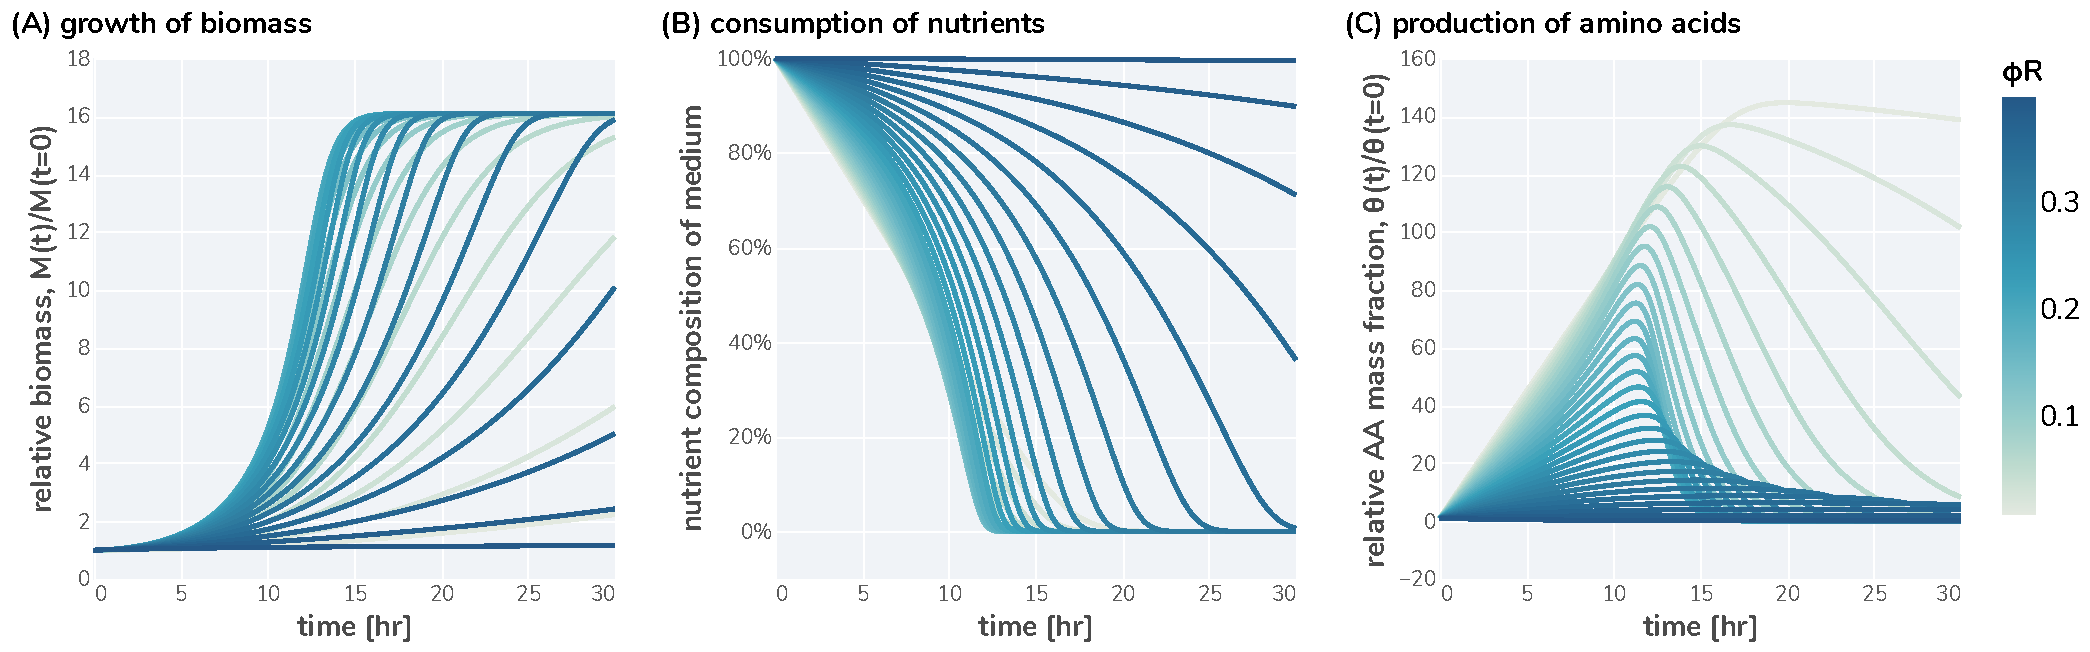
\includegraphics[width=\textwidth]{figures/single_nutrient_dynamics.pdf}
\caption{\textbf{Dynamics of growth on a single nutrient source.} (A) Biomass of
the system relative to the initial condition $M(t=0)$. (B) The fractional
concentration of the nutrients in the growth medium relative to that of $c(t =
0)$. (C) The relative mass fraction of amino acids $\theta_a$ relative to
$\theta_a(t = 0)$. For all plots, parameters were chosen to be approximately
similar to growth of \textit{E.  coli} on a glucose-based medium. Explicitly,
the model parameters used here are $\phi_R^{(max)} = 0.4$, $\gamma^{(max)} =
8.25\,\text{hr}^{-1}$, $\nu^{(max)} = 2.5\,\text{hr}^{-1}$, $\theta_0 = 0.002$,
$c = 50\,\text{mM}$, $\Omega = 0.3$, and $K_M = 5\,\mu\text{M}$. The initial 
conditions were arbitrarily set to be $M_0 = 0.001$ and $\theta_a =
\frac{M_0}{10}$.}
\label{fig:single_nutrient}
}
\end{figure}
\subsection{Growth on Two Carbon Sources}
Given a dynamical model of growth on a single nutrient source, it becomes
relatively simple to include the presence of a second nutrient source whose 
metabolism is not preferred. 

Let us consider two nutrient sources $x$ and $y$. Nutrient $x$ is the
"preferred" nutrient, meaning that its metabolism is prioritized over $y$.
The As $x$ and $y$ are different substrates, they require different sets of
metabolic proteins $M_x$ and $M_y$ and corresponding proteome mass fractions
$\phi_x$ and $\phi_y$. Additionally, as the nutrients are different, so too
are the nutritional capacities $\nu_x$ and $\nu_y$ which are determined given
the concentrations $c_x$ and $c_y$ and Monod constants $K_{M,x}$ and
$K_{M,y}$, respectively. The translational capacity, however, is shared
between the two nutrient sources as it is dependent only on the amino acid
pool $\theta_a$ resulting from the metabolism of $x$ or $y$.

How do we define a "preferred" substrate? In order to regulate what is
metabolized, we must think of how the expression of the metabolic proteins are
regulated. We will begin by considering that the expression of the metabolic
proteins responsible for consuming each the preferential nutrient $x$ will be 
proportional to its concentration $c_x$. Mathematically, we can model the mass
fraction $\phi_x$ to have Monod-like dependence on the concentration $c_x$,
yielding 
\begin{equation}
\phi_x(c_x) = \frac{\phi_x^{(max)}}{1 + \frac{K_{M, x}}{c_x}}. 
\label{eq:phix_monod}
\end{equation}


















\end{document}